\chapter{Proposta de extensão}\label{chp:extensao}

No decorrer dos dois anos de desenvolvimento do projeto, buscou-se a formação no campo de desenvolvimento de aplicações, comunicação via \textit{socket}, aprendizado de \textit{Unity}, aprofundamento em visão computacional e, principalmente, pesquisa bibliográfica em aplicação de realidade aumentada em neurocirurgias. Contudo, toma-se a abordagem da aplicação dos óculos \textit{Moverio BT-350} como ferramenta auxiliar de visualização anatômica do paciente em tempo real durante uma neurocirurgia. Para isso, foi proposto uma arquitetura compatível com equipamentos disponíveis e com tempo de resposta adequado.

No momento, o projeto funciona da maneira esperada, porém com muito espaço para ser aperfeiçoado antes de ser levado para a avaliação dos médicos. Os quesitos que podem ser melhorados são:

\begin{description}
   \item[Método da Detecção de Posição:] O projeto utiliza somente um marcador \textit{ArUco} para estimar sua posição, o que traz principalmente o problema do usuário perder o marcador de vista por causa do ângulo de observação.
   \item[Otimização da latência do sistema:] Os fatores que limitam o tempo de resposta do sistema é principalmente a conexão sem fio dos óculos com o \textit{access point} e do roteador até o servidor.
\end{description}

A solução desses fatores torna a pesquisa apresentável para os médicos do Centro de Cirurgia de Epilepsia (CIREP) do Hospital das Clínicas da Faculdade de Medicina de Ribeirão Preto-USP. A parceria aproxima dos integrantes do laboratório dos pesquisadores do CIREP em forma de reuniões \textit{online} e eventuais visitas até o hospital das clínicas. Seguindo essa oportunidade, se forem preparadas demonstrações do \textit{VCranium}, o projeto pode receber sugestões diretas dos médicos e compiladas em um artigo científico. 

\section{Objetivo}

Otimizar os processos do sistema de reconhecimento de posição da cabeça do paciente; definir um método de reconhecimento mais robusto e que permita demonstrações. Por fim, apresentar o projeto aos pesquisadores do Centro de Cirurgia de Epilepsia do Hospital das Clínicas da Faculdade de Medicina de Ribeirão Preto-USP.

\section{Metodologia}

O projeto já possui uma arquitetura que permite a alteração da forma de final de reconhecimento da pose de uma cabeça humana. Dessa forma, alterar o método de detecção de \textit{ArUco} pode ser feito sem problemas. A confiabilidade comprovada do métodos dos marcadores pode ser ampliada com o uso mais marcadores, criando uma maior cobertura de atuação do sistema.

\begin{figure}[ht]
    \centering
    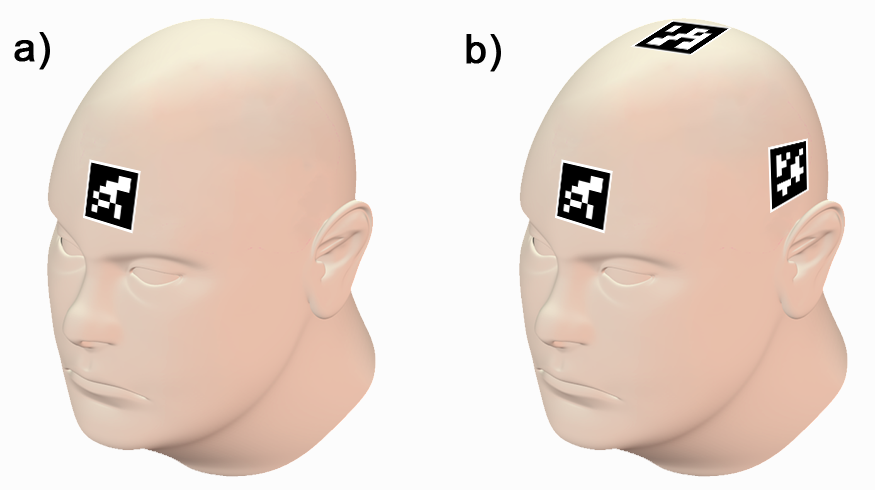
\includegraphics[width=.6\linewidth]{figuras/head_marker.png}
    \caption{a) Aplicação atual de marcadores no projeto. b) Exemplo de utilização de múltiplos marcadores. Fonte: Autor.}
    \label{fig:head-markers}
\end{figure}

Atualmente, o projeto aplica os marcadores como na Figura \ref{fig:head-markers}a. Dessa forma, o sistema está limitado a estimar a posição da cabeça somente em sua face frontal, i.e., não identifica as laterais e face traseira da cabeça. Uma solução para esse problema é proposto na Figura \ref{fig:head-markers}b, que invés de um único marcador, múltiplos marcadores são colocados em todas os lados da cabeça, com a de reconhecer a sua posição independentemente em cada marcador.

% A aplicação atual de marcadores do projeto pode ser vista na Figura \ref{fig:head-markers}a. Podemos observar que o sistema pode estimar a posição da cabeça em somente sua parte frontal, portanto, o sistema não funciona se observamos as laterais e atrás da cabeça. A Figura \ref{fig:head-markers}b traz uma solução a esse problema posicionando 5 marcadores em todos os lados da cabeça, assim o sistema pode estimar a posição do cérebro individualmente (Figura \ref{fig:tiara}).

\begin{figure}[ht]
    \centering
    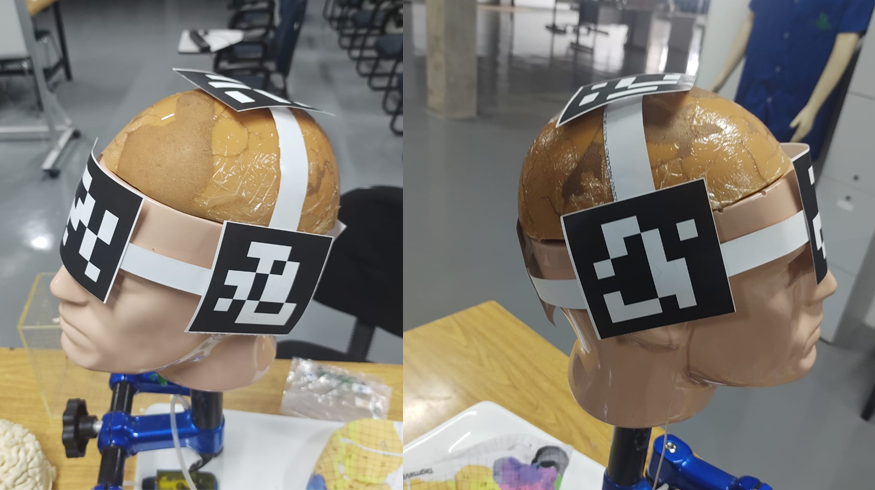
\includegraphics[width=.6\linewidth]{figuras/tiara.png}
    \caption{Esboço de uma tiara que suporta um marcador em cada lado da cabeça. Fonte: Autor.}
    \label{fig:tiara}
\end{figure}

Uma forma de posicionar múltiplos marcadores é utilizar uma "tiara" para portá-los, um esboço desse objeto foi construído com papel na Figura \ref{fig:tiara}. Esse método utiliza transformações de base, fundamentados da disciplina de Geometria Analítica e Álgebra Linear, para a estimar a posição central da cabeça e sua orientação. Para isso, deve-se saber a posição e orientação de cada marcador em relação ao centro da cabeça e, visto que os tamanhos da cabeça variam, encontra-se a necessidade de uma calibração para cada paciente. Pensando na impossibilidade do contato direto do marcador com a pele do paciente e a possível oclusão do marcador por ferramentas e as mãos do médico, esse método se torna uma opção menos viável para situações cirúrgicas.

Uma solução alternativa seria utilizar múltiplos marcadores distantes do pacientes, mas ainda visíveis na câmera dos óculos como na Figura \ref{fig:cube}. Os marcadores em formato de cubo facilitam e a montagem a calibragem de cada marcador em relação ao centro da cabeça.

\begin{figure}[ht]
    \centering
    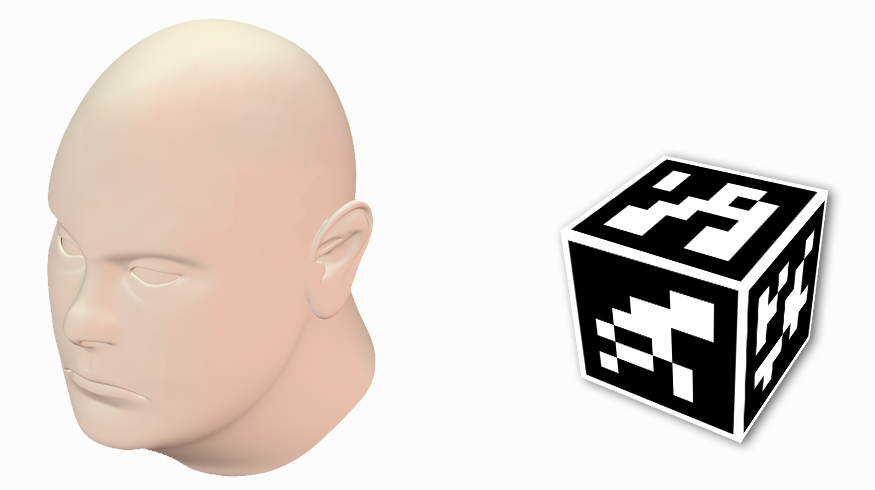
\includegraphics[width=.6\linewidth]{figuras/cube.png}
    \caption{Solução de estimação de posição com cubo de marcadores. Fonte: Autor.}
    \label{fig:cube}
\end{figure}

Por fim, o projeto vai aproveitar o tempo de extensão para fazer um pedido de Bolsa Estágio de Pesquisa no Exterior (BEPE) para buscar cooperação com grupos de pesquisa do exterior. O intercâmbio, além de colocar a comunicação acadêmica em prática, tem a oportunidade de receber críticas aprofundadas e criativas no assunto de realidade aumentada, visto que muito desses equipamentos são raramente vendidos no Brasil.

\newpage

\section{Cronograma}

O controle de atividades vai ser feito com encontros mensais e semanais com o coorientador, orientador e integrantes do laboratório. Um cronograma foi elaborado na tabela \ref{fig:tabela} para servir de guia para o progresso do projeto.

\begin{table}[h]
    \centering
    \begin{tabular}{lllllll} 
            \hline
        \multicolumn{7}{c}{\textbf{Cronograma de atividades para a extensão}} \\ 
            \hline
        & & {\cellcolor[rgb]{1,.3,.3}} & \multicolumn{4}{l}{Execução} \\ 
            \hline
        \textbf{Atividade} & \textbf{Bimestre} & 1 & 2 & 3 & 4 & 5\\ 
            \hline
        Programação dos novos métodos com marcadores & & {\cellcolor[rgb]{1,.3,.3}} & & & & \\ 
            \hline
        Montagem dos protótipos de tiara e cubo & & {\cellcolor[rgb]{1,.3,.3}} & {\cellcolor[rgb]{1,.3,.3}} & & & \\ 
            \hline
        Estudos no exterior (BEPE) & & & & {\cellcolor[rgb]{1,.3,.3}} & {\cellcolor[rgb]{1,.3,.3}} & \\ 
            \hline
        Produção de relatório final e relatório BEPE & & & & & & {\cellcolor[rgb]{1,.3,.3}}\\ 
            \hline
        Apresentação final do trabalho* & & & & & & {\cellcolor[rgb]{1,.3,.3}}  \\
            \hline
    \end{tabular}
    \caption{*A apresentação para os pesquisadores da parceria do Centro de Cirurgia de Epilepsia (CIREP) do Hospital das Clínicas da Faculdade de Medicina de Ribeirão Preto-USP}
    \label{fig:tabela}
\end{table}